% Template article for document class `jicspack'
% 2004/10/07


\documentclass[print]{jicspack}
\setvolume{11}                             %for printing use only
\setyear{2015}                             %for printing use only
\setpagerange{1}{8}                    %for printing use only
\setheadauthor{X. Liu et al.}          %for printing use only
\setissn{1553--9105} \setpubdate{January 2015} \setno{1}

\afterpage{\beginheader}                   %for printing use only


\usepackage{enumerate}
% if you use PostScript figures in your article
% you can use the graphics package
% \usepackage{graphics}
% or use the graphicx package for more complicated function
\usepackage{graphicx}
% or use the epsfig package
% \usepackage{epsfig}

% The amssymb package provides various useful mathematical symbols
\usepackage{amssymb}

\begin{document}

\begin{premaker}

% The premaker environment contains Title, authors and addresses;
% use the thanksref command within \title, \author or \address for footnotes;
% use the corauthref command within \author for corresponding author footnotes;
% use the ead command for the email address,
% and the form \ead[url] for the home page:
% \title{Title\thanksref{label1}}
% \thanks[label1]{}
% \author{Name\corauthref{cor1}\thanksref{label2}}
% \ead{email address}
% \ead[url]{home page}
% \thanks[label2]{}
% \corauth[cor1]{Corresponding author}
% \address{Address\thanksref{label3}}
% \thanks[label3]{}

\title{An Improved Imputation Algorithm Based on QENNI \thanksref{label1}}
\thanks[label1]{Project supported by the National Nature Science Foundation of China (No. ***).}
\author[author1]{Zhibo Chen\corauthref{cor1}},
\ead{zhibo@bjfu.edu.cn}
%\thanks[label2]{Footnotes for authors}
\corauth[cor1]{Corresponding author.}
% other authors
\author[author2]{JianXin Wang},
\author[author3]{Zhaoyu Zhang},
\author[author4]{Qiuwu Yuan},

\address[author1]{School of Information Science And Technology, Beijing Forestry University, Beijing 100083, China}
\address[author2]{School of Information Science And Technology, Beijing Forestry University, Beijing 100083, China}
\address[author3]{School of Information Science And Technology, Beijing Forestry University, Beijing 100083, China}
\address[author4]{School of Information Science And Technology, Beijing Forestry University, Beijing 100083, China}
%\thanks[label3]{Footnotes for address}
% you can use optional labels to link authors explicitly to addresses:
% \author[label1]{},
% \author[label2]{}
% \address[label1]{}
% \address[label2]{}

\begin{abstract}
% Text of abstract
Missing data imputation is an important research aspect in data mining. Data quality is a major concern in Machine Learning and other correlated areas such as Knowledge Discovery from Databases (KDD). Many imputation methods of missing data have been designed to resolve the problem. More or less, they have some deficiencies. As the K-Nearest Neighbor Imputation ($k$NNI) Algorithm is often biased in choosing the $k$ nearest neighbors of missing data. A new imputation method is put forward, Quadrant Encapsidated Nearest Neighbor based Imputation method (QENNI). QENNI uses the quadrant nearest neighbors around a missing datum to impute the missing data value. It is not biased in selecting nearest neighbors. Experiments demonstrate that QENNI is much better than the $k$NNI method in imputation accuracy. But, as the experiments proceed, we find out the density of points in each quadrant and the distance between the two point affect the missing data value seriously. So, we improved the QENNI algorithm and put forward Density and Distance Weighted Quadrant Encapsidated Nearest Neighbor based Imputation method algorithm (DDWQ). The experimental result demonstrates that our DDWQ method has a higher imputation accuracy than QENNI.
\end{abstract}
\begin{keyword}
% keywords here, in the form: keyword \sep keyword
Imputation of missing data \sep Quadrant \sep Shell-neighbors  \sep $k$NNI \sep QENNI \sep DDWQ
\end{keyword}
\end{premaker}

% main text
\section{Introduction}
\label{Maintext}
Data mining is an interdisciplinary subfield of computer science. It is the computational process of discovering patterns in large data sets involving methods at the intersection of artificial intelligence, machine learning, statistics, and database systems. The overall goal of the data mining process is to extract information from a data set and transform it into an understandable structure for further use. Data mining is a powerful technology with great potential. Pre-processing as one of the indispensable step of data mining can seriously affect the accuracy of the conclusion. That is why missing data imputation has been an inevitably and challenging research.

Due to its importance in data mining, missing data imputation has received considerable attention during the past decades. A large percentage of studies\cite{Research1,Research2,Research3,Research4,Research5} have been done to develop procedures to deal with missing values. Recently, no matter in which field of study, $k$NNI\cite{KNNI2,KNNI3,KNNI4} imputation method has been researched and applied widely because of its easy operating, high efficiency and accuracy. It is an excellent imputation algorithm, but those choosing nearest neighbors of missing data is very likely biased on one side. So it's not the best choice to use them for missing data imputation. In addiction, the parameter $k$ is the key factor for the $k$NNI algorithm. In the experiments, if the $k$ sets a larger value, it brings seriously randomness; if the $k$ sets a smaller value, it will lose large sample size standard of statistics. Before very experiment of $k$NNI, lots of calculation should be token to get the appropriate value of $k$. It makes the algorithm more complex. In response to these problems, Shichao Zhang put forward the Shell-neighbors\cite{Shell} viewpoint of missing data imputation and realize a new missing data imputation algorithm, quadrant encapsidated nearest neighbor based imputation (QENNI). QENNI algorithm imputes the missing data by finding all of the quadrant encapsidated nearest neighbors of the missing data. Exactly to say, it assumes the incomplete data as the center, the complete data sets are distributed to each quadrant. Because of this feature, it can void the heavily depending on the parameter $k$ of $k$NNI. Experimental results show QENNI has a higher accuracy than $k$NNI.

But, according to the analysis of the incomplete data, we find it also seriously affected by density of points in each quadrant and the distance between the incomplete data and complete data. So, based on QENNI,  we take the density and distance's weight into account and propose a new missing data imputation algorithm, Density and Distance Weighted Encapsidated Nearest Neighbor based Imputation method (DDWQ). This imputation algorithm overcomes the above-mentioned limitations and has a good performance than QENNI.

The rest of this paper is organized as follows: Section 2 introduces the details of the proposed imputation method and give the corresponding algorithm. Section 3 gives the experiments and results. Section 4 discusses the result and draws a conclusion.

\section{DDWQ Algorithm}
\label{sec:2.1}
On the basis of the above discussion, in this part, we give the definition and implementation of the DDWQ algorithm and point out the improvement of DDWQ algorithm. We also discuss the shortcomings of $k$NNI and QENNI algorithm.
\subsection{Algorithm background}
Suppose $X$ is an M-dimensional random vector, $Y$ is the dependent variable affected by $X$. In practice, if a missing data random sample (size is $n$) can be get, it can be expressed as $(X_i, Y_i, \delta_i), i= 1, 2,\cdots, n$. In which, all of the $X_i$ vector is observable, when $Y_i$ is missing, $\delta_i = 1$, otherwise $\delta_i = 0$. If the data set $T$ contains $n$ data, each data has $m + 1$ attributes (contains $m$ condition attributes and $1$ decision attribute), keep: $T_i = (X_{i1}, X_{i2}, \cdots, X_{im}, Y)$ (missing values are generated only in decision attribute $Y$). $T = I \bigcap C$, let $r = \sum\limits_{k=1}\limits^{n} \delta_i$, $I = {T_1, \cdots, T_r}, r \leq n$ are the data sets which decision attributes are missing, referred to missing datasets; $C = {T_r+_1, \cdots, T_n}$ is the complete datasets.
\subsection{$k$NNI algorithm}
\label{2.2}
K-Nearest Neighbor Imputation ($k$NNI) Algorithm imputes the missing value by the $k$ nearest neighbors of the incomplete data. It bases on the theory that the closer the distance, the closer the relation. If a data loses one attribute, to find out the $k$ nearest neighbors in complete data sets and use the average value of them to impute the missing value.

As previously mentioned, $k$NNI is praised by the majority of researchers because of its simple operation, low time complexity and high imputation accuracy. But there are still some drawbacks. The $k$ nearest neighbors selected by $k$NNI algorithm may occur preferences, which makes the filling result relatively inefficient. In fact, from the distribution of complete data which surrounds the missing data, the distribution of its nearest neighbors and overall data may be inconsistent. For instance, as shown in Fig.\ref{fig:figure1}, $O$ represents missing data, the other points represents complete data, we use $k$NNI algorithm to impute the missing data value. According to the way of $k$NNI, we need to find three nearest neighbors and use them to impute the missing data value. So $A, B, C$ are selected. Nevertheless, from Fig.\ref{fig:figure1} we can clearly see that the complete data surrounding the missing data are evenly distributed, but the three selected nearest neighbors bias in the first quadrant. So the three nearest neighbors may not be the best choice and we can't get the best results by using them to impute the missing value.

\begin{figure}[h]
\centering
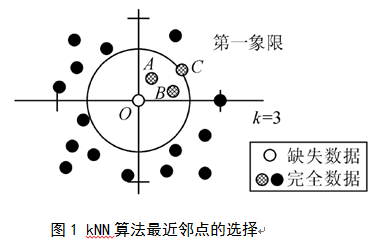
\includegraphics[angle=0, width=0.4\textwidth]{figure1.png}
\caption{Nearest neighbors chosen by $k$NN}
\label{fig:figure1}
\end{figure}

To choose the $k$ parameter of $k$NNI algorithm is difficult. Each time, we use $k$NNI to impute the missing data, we need to repeat the experiment so many times to obtain the value $k$. Once the value of $k$ occurs deviation, the performance of $k$NNI will be significantly lower. In conclusion, if the imputation algorithm can eliminate the dependence on the parameter $k$, it will be the best choice.

\subsection{QENNI algorithm}
\label{2.3}
We propose the hypothesis that the complete data which is used to impute missing data must be the nearest neighbors and in the first encirclement of the incomplete data. we also need to eliminate the dependence on the parameter $k$. Let's realize the idea below.

\begin{figure}[h]
\centering
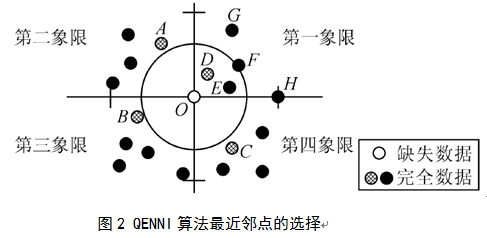
\includegraphics[angle=0, width=0.4\textwidth]{figure2.png}
\caption{Nearest neighbors chosen by QENNI}
\label{fig:figure2}
\end{figure}

\begin{enumerate}[(1)]
\item First, take data $(X_i, X_2, \cdots, X_m)$ which contains $m$ condition attributes as a point of $m$-dimensional space, establish a coordinate system and the missing data is the center. Through the axis to divide the $m$-dimensional into $2^m$ quadrants.
  \begin{enumerate}[a.]
  \item When $m = 2$, the condition attributes $(X_1, X_2)$ can be regarded as a point of plane. As shown in Fig.\ref{fig:figure2}, the axis divides the plane into $2^2$ quadrants. If one point is just between the two quadrants, we classify it to one of its nearby quadrant. According to our definition, each of the complete data can be located in the only certainty quadrant.
  \item Similarly, when $m = 3$, the condition attributes of data is $(X_1, X_2, X_3)$. The formed spatial coordinate system divides the space into $2^3$ quadrants and each of the complete data is also in the only identified quadrant.
  \item Extended to the general case, when $m = m$, the condition attributes of data is $(X_i, X_2, \cdots, X_m)$ and the space is divided into $2^m$ quadrants.
  \end{enumerate}
\item Based on the dividing of $m$-dimensional space, the Euclidean distance of each point (complete data) from its own to the center (which is the incomplete data) is calculated. To find out the nearest one of each quadrant (if not exists, ignore it) and use decision attributes of them to impute the missing data value. With $m = 2$, for example, as shown in Fig.\ref{fig:figure2}. In each quadrant,  we select $A, B, C, D$ as the nearest neighbors and use the decision attributes $Y$ of them to impute the missing data value of center $O$. It also weighted by the distance of each selected point. Obviously, the result of QENNI to choose the nearest neighbors is different from the $k$NNI algorithm.
\begin{equation}
\label{eq:1}
dist(T_i, T_j) =\sqrt{ \sum\limits_{k=1}\limits^{m} (X_{ik} - X_{jk})^2}
\end{equation}
\item In order to analyze the effectiveness of the algorithm better, for each missing data $T_i (T_i \in I)$, on the basis of QENNI algorithm,  the following definition can be given:
\begin{defn} The coordinate system centered at $T_i$ divides the space into $2^m$ quadrants and the complete dataset $C$ based on quadrant is divided into $2^m$ subset $C = \{D_1, D_2, \cdots, D_q, \cdots, D_{2^m}\}$. Each complete data set $D_q (q = 1, 2, \cdots, 2^m)$ is the $q$ quadrant's data of $T_i$. \end{defn}
\begin{defn} $\forall T_j \in D_q$, satisfy $Near_q = \arg \min dist_{T_j \in D_q}(T_i, T_j)$, $Near_q$ is the nearest neighbor of $T_i$ in $q$ quadrant. As shown in Fig.\ref{fig:figure2}, the first quadrant data of $T_o$ is $D_1 = \{T_D, T_E, T_F, T_G, T_H \}$. So $Near_q = T_D$ which is the nearest neighbor of the first quadrant. \end{defn}
\begin{defn} In the $q$ quadrant, take $T_i$ as the center of the sphere (or hypersphere), dist($Near_q, T_i$) as the radius to ensure the $Shell_q$ of $T_i$ in $q$ quadrant. \end{defn}
\begin{defn} All of the $Shell_q (q = 1, 2, \cdots, 2^m)$ and axis constitute the $m$-dimensional subspace which is Shell of $T_i$. \end{defn}
\begin{defn} All the of nearest neighbors $\{Near_1, Near_2, \cdots, Near_{2^m}\}$ of $T_i$ in each quadrant are called the points of Shell. \end{defn}
\begin{col} If $D_q \neq \O$, the Shell of $T_i$ must exists in $q$ quadrant.\end{col}
\begin{col} $\forall T_j \in D_q$, $\exists dist(T_j, T_i) \geq dist(Near_q, T_i)$. \end{col}
\item In summary, the QENNI algorithm can overcome the shortcomings of $k$NNI in choosing the $k$ nearest neighbors of missing data. The selected complete data is not biased in any side and the Shell of the missing data is smallest. That is to say it does not exist any other complete data on the Shell of the missing data. It is thus clear that QENNI algorithm can find out the most satisfied complete data without any preferences. They can represent the missing data value better than $k$NNI.
\end{enumerate}

\subsection{DDWQ aglorithm}
\label{2.4}
Even though the QENNI algorithm has a better performance than $k$NNI, it does not take the density of complete data in each quadrant into account. As shown in Fig.\ref{fig:figure3}, if we just think about the distance of complete data $A$ and $D$, the $D$ has a higher effect of the result. But it is clearly that just the distance can not represents the real effect of the complete data $A$. If the density of complete data surrounding $A$ is token into account, it may have a higher weight than $D$. Based on the above considerations, our new algorithm takes both the weight of distance and density into account. The following definitions are given.
\begin{figure}[h]
\centering
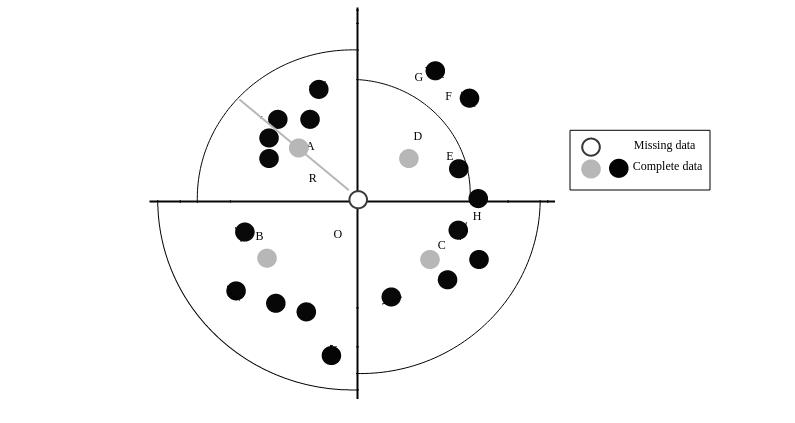
\includegraphics[angle=0, width=0.5\textwidth]{figure3.png}
\caption{Nearest neighbors chosen affected by Density}
\label{fig:figure3}
\end{figure}

\begin{enumerate}[(1)]
\item Weight of Distance : The different length of distance has different size of influence. The more closer, the higher weight. So we keep weight of each nearest neighbor $Near_i (i=1, 2, \cdots, 2^m)$ in every quadrant as:
\begin{equation}
\label{eq:2}
W(D)_i = \frac{1}{dist(Near_i, T_i)^2}
\end{equation}
\item Weight of Density : The density represents the number of complete data in per unit volume and it can indicate the wight of the quadrant's density. We use Eq. (\ref{eq:3}) to calculate the volume of n-sphere. The Eq. (\ref{eq:5}) is used to calculate the density which can represents the weight. Each quadrant's number of complete data in the limited volume of n-sphere which has $R \leq 2 * dist(Near_i, I_i)$ is counted as $N = \{N_1, \cdots, N_i, \cdots, N_{2^m}\}$.

\begin{equation}
\label{eq:3}
V_n(R) = \frac{\pi^{\frac{n}{2}}R^n}{\Gamma (\frac{n}{2} + 1)}
\end{equation}

\begin{eqnarray}\label{eq:4}
\Gamma(\frac{n}{2} + 1) = \left\{\begin{array}{ll}(\frac{n}{2})! & \mbox{n is even} ,\\\sqrt{\pi}\frac{n!!}{2^{\frac{n+1}{2}}} & \mbox{n is odd}.\end{array}\right.
\end{eqnarray}

\begin{equation}
\label{eq:5}
W(\rho)_i = \frac{N_i}{\frac{V_n(R)_i}{2^m}}
\end{equation}

\item Core algorithm : The algorithm takes both density and distance's weight into consideration and bring in the factor $\beta (0.0 \leq \beta \leq 1.0)$ to decide the percentage of density and distance.  The followings are the detailed steps of DDWQ :
\begin{enumerate}[a.]
  \item Calculate the Euclidean distance of missing data set $I$ and complete data set $C$ by Eq. (\ref{eq:1}).
  \item Iterate data set $I$ and $C$, calculate the nearest neighbors, total number of complete data in each quadrant where $R \leq 2 * dist(Near_i, I_i)$ and volume of each hyperspace by Eq. (\ref{eq:2}, \ref{eq:3}, \ref{eq:5}).
  \item The key about how to figure the complete data for each quadrant is to translate the data vector into a number and use it to mark the quadrant. First, translate the coordinate into a vector consisting of one and zero. if the value of vector greater than zero, translate it into one, otherwise keep it as zero. Than, translate the binary number into decimal number and use it to mark the quadrant.
  \begin{equation}
  \label{eq:6}
  \begin{pmatrix} 2& -1& 0\end{pmatrix}\Rightarrow \begin{pmatrix} 1& 0& 0\end{pmatrix} \Rightarrow (1*2^2 + 0*2^1+ 0*2^0) \Rightarrow 4
  \end{equation}
  \item Take the previous results into Eq. (\ref{eq:7}) to calculate the missing data value ($v_i$). The equation has token the weight of density and distance into account.
  \begin{equation}
  \label{eq:7}
  v_i = \frac{\sum\limits_{i=1}\limits^{n}((1-\beta)W(D)_i + \beta W(\rho)_i) * D_i}{\sum\limits_{i=1}\limits^{n}((1-\beta)W(D)_i + \beta W(\rho)_i}
  \end{equation}
\end{enumerate}
\end{enumerate}

\section{Experiments and Results}
\subsection{Dataset}
\label{sec:1.1}
In order to test our algorithm, we choose the open datasets Abalone which is from UCI and Delta\_ailerons which is from weka. We do the same experiments as QENNI does. The sex attribute is excluded and left the data whose sex value is $M$. It has 8 attributes and 1528 records in total. The Diameter attribute is chosen as decision attribute and missing data is generated on it. The Delta\_ailerons dataset has 6 attributes and 7129 records in total. The last attribute is chosen as decision attribute and the missing data is generated on it. The imputation accuracy is used as evaluation index. In general, the Root Mean Square Error (RMSE)\cite{RMSE} is used. $e_i$ is the original value, $e'_i$ is the imputation value and $m$ is the number of missing data. The smaller the RMSE, the higher the imputation accuracy.
\begin{equation}
\label{eq:6}
RMSE = \frac{1}{m}\sum\limits_{1=1}\limits^{m}(e_i - e'_i)^2
\end{equation}

\subsection{Experiments and results analysis}
In order to get more objective results, both datasets randomly generate the missing data. For evaluation, the missing rate sets $5\%$ and 200 times of random missing experiments are done on it to calculate the average of RMSE. The following is the comparison of QENNI and WWDQ when $\beta \in \{0.0, 0.1,\cdots,  0.5,\cdots, 1.0\}$.

\begin{figure}[h]
\centering
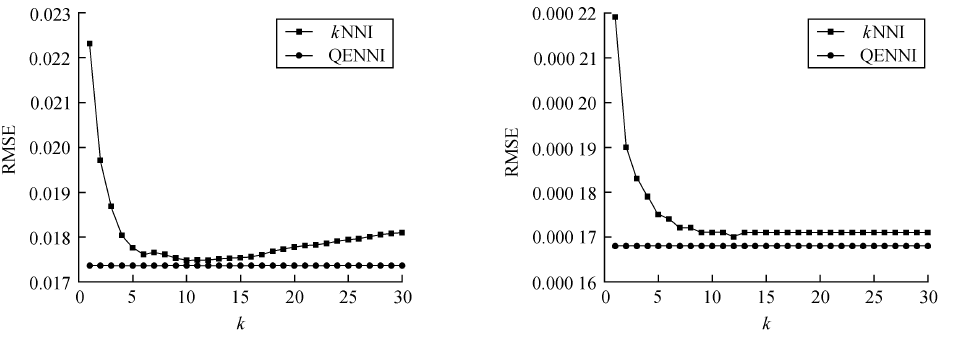
\includegraphics[angle=0, width=0.8\textwidth]{figure4.png}
\caption{Comparison of the Two Algorithm}
\label{fig:figure4}
\end{figure}
Compared from the Fig. \ref{fig:figure4}, we can draw a conclusion that WWDQENNI algorithm has better imputation accuracy than QENNI no matter what's the value of $\beta$.

\section{Conclusion}
For improving the accuracy of missing data imputation, DDWQ imputation algorithm has been put forward. The algorithm is able to overcome the limitations of $k$NNI and QENNI. The innovation of our algorithm is to take the density of points in each quadrant and distance between the complete data and the missing data into consideration based on the Shell-neighbors thought. So, the result of missing data value can be more closer to the ideal one. The experimental results indicate that DDWQ algorithm has a better performance than QENNI.

\begin{thebibliography}{00}\label{ref:ref}

% \bibitem{label}
% Text of bibliographic item

% notes:
% \bibitem{label} \note

% subbibitems:
% \begin{subbibitems}{label}
% \bibitem{label1}
% \bibitem{label2}
% If there is a note, it should come last:
% \bibitem{label3} \note
% \end{subbibitems}


\bibitem{Research1} Zou G H, Li Y F, Zhu R, et al. Imputation of mean of ratios for missing data and its application to PPSWR sampling[J]. Acta Mathematica Sinica, English Series, 2010, 26(5):863-874.
\bibitem{Research2} Zhang S, S Z, Zhang S, et al. Missing Value Imputation Based on Data Clustering[J]. Lecture Notes in Computer Science, 2008:128-138.
\bibitem{Research3} Luengo J, Saez J A, Herrera F. Missing data imputation for fuzzy rule-based classification systems[J] . Soft Computing, 2012, 16(5):863-881.
\bibitem{Research4} Zhang S, S Z, Zhang S, et al. Missing data imputation by utilizing information within incomplete instances[J]. Journal of Systems and Software, 2011, 84:452-459.
%\bibitem{Research5} Feng-mei W, W F, Feng-mei W, et al. A Missing Data Imputation Method Based on Neighbor Rules[J]. Computer Engineering, 2012.
\bibitem{Research5} P. Smaragdis, B. Raj, and M. Shashanka, Missing data imputation for spectral audio signals, in IEEE Workshop in Machine Learning for Signal Processing (MLSP), 2009.
\bibitem{Shell} Zhang, S. (2011). Shell-neighbor method and its application in missing data imputation. Applied Intelligence, 35, 123-133.
%\bibitem{KNNI1} Li, D., Deogun, J.S., Spaulding, W., Shuart, B.: Towards missing data imputation: A study of fuzzy k-means clustering method. In: S. Tsumoto, R. Slowinski, J. Komorowski, J.W. Grzymala-Busse (Eds.), Proceedings of the 4th International Conference on Rough Sets and Current Trends in Computing.Lecture Notes in Artificial Intelligence 3066, Uppsala, Sweden, Springer-Verlag Berlin (2004) 573-579.
\bibitem{KNNI2} Ling, Wang, Fu Dong-Mei. Estimation of Missing Values Using a Weighted K-Nearest Neighbors Algorithm. Environmental Science and Information Application Technology, 2009. ESIAT 2009. International Conference on. IEEE, 2009:660-663.
\bibitem{KNNI3} BATISTA G E, MONARDMC . A study of k-nearest neighbor as a model-based method to treat missing data[C] Proceedings of the Argentine Symposium on Artificial Intelligence. Bering Germany : Springer, 2001, 30: 1-9.
\bibitem{KNNI4} Kung Y, et al. An optimal k-nearest neighbor for density estimation[J]. Statistics \& Probability Letters, 2012, (10):1786-1791.
\bibitem{RMSE} Aptula A, Jeliazkova N, Schultz T, et al. The Better Predictive Model: High q 2 for the Training Set or Low Root Mean Square Error of Prediction for the Test Set?[J]. Qsar \& Combinatorial Science, 2005, 24(3):385-396.
% \bibitem{QENNI} 张师超, 朱曼龙, & 黄樑昌. (2010). Qenni:一种缺失值填充的新方法. 广西师范大学学报:自然科学版, 28, 1.
\end{thebibliography}

\end{document}
